\section{Designing FSO Devices for Flexible Inter-Rack Networking}
\label{sec:fso}

In this section, we begin by specifying the design requirements for
FSO devices in \ArchName, and then describe our design roadmap for
meeting these requirements.

\subsection{Overview and Requirements}

The design of FSO devices in \ArchName must simultaneously meet
the following requirements:

\begin{packeditemize}
\item {\em Size, cost-effectiveness, and power:} A single FSO device
  assembly (i.e., including steering and alignment machinery) should
  have a footprint of $\approx$ $3" \times 8"$, so that a few tens of
  them can be placed on the ToR. Each device shouldn't cost much more
  than \$1000, for our overall design to be
  cost-effective~\cite{hotnets}.  Finally, their power consumption
  should be modest.

\item {\em High (10-100Gbps) data rate over long distances (50-100m),
  with a ``misalignment-tolerance'' of about 4mm:} DC traffic rates
  are growing~\cite{ananta}, and inter-rack distances in large DCs can
  easily be of the order of 50-100m~\cite{dc-size}.  Thus, FSO links
  must be capable to providing high throughput over such distances.
  Finally, we would like the links to be able to tolerate minor
  misalignments (between TX and RX) due to rack vibrations, airflow
  shifts, etc.

\item {\em Fast and precise alignment and steering:} For efficient
  communication, the transmit/receive devices must be precisely
  aligned. Thus, we need mechanisms for robust re-aligment in face of
  environmental effects such as vibrations or changes in airflow.
  Furthermore, to provide fine-grained and efficient
  reconfigurability, we need a mechanism to precisely steer the
  \blue{laser} beam (in order of tens of msecs~\cite{hotnets}) to
  connect to another FSO device.
\end{packeditemize}

% existing solutions suck
Unfortunately, commercially available FSO transceivers are very bulky
(up to 2 cubic feet of volume~\cite{}), expensive (\$6-15K for a
single device), and power hungry (tens of watts). This is because they
target outdoor long distance (many miles) communications~\cite{}, and
hence, require additional mechanisms to overcome environmental
factors~\cite{} and long distances. These issues largely disappear in
the context of indoor DCs; but, we also have an additional requirement
of fast steering.

Next, we outline our plan to design an FSO device that meets the above
requirements. We first address the first two requirements, and then,
address choice and design of alignment/steering mechanisms.

\subsection{Cost-Effective, Small-Form Factor, and High-Throughput FSO Devices}

\begin{task}
We will design FSO devices that satisfy the size, power, cost, and
throughput requirements. We will investigate the size and cost
vs.\ performance tradeoff in a DC-specific context.
\end{task}

\smallskip

%% basic idea -- SFP to FSO, why? Challenges therein.
\para{Converting Optical SFPs to FSOs.}  An FSO communication link has
three basic components: (i) a modulated laser source (typically
infrared) as a transmitter (TX); (ii) a high-speed optical
detector/demodulator receiver (RX); and (iii) a robust optical path
between TX and RX.
%
To demonstrate feasibility of a small and cost-effective FSO link, we
would build an FSO link using the commodity optical SFP (small
form-factor pluggable) transceivers~\cite{}. Optical SFPs are widely
used to interface optical fibers with (electrical) packet switches.
They are small ($1'' \times 2'' \times 3''$) and low-cost
(\$100-200). FSOs based on optical SFPs would easily satisfy our size,
cost, and datarate requirements, and would not create an additional
power burden since SFPs are likely to be used for high-throughput
links in DCs anyway.
%
The key difference between optical SFPs and FSOs is that in SFPs, the
laser beam is launched directly into the fiber, while in FSOs, the
laser beam would be launched into free space.
%
While the idea of converting SFPs to FSOs has been addressed
before~\cite{mustafa2013reintroducing}, the context of DCs brings in
new challenges.
%
The main challenges that arise in converting an SFP into an FSO link
are (i) minimizing beam divergence, and (ii) need for precise
alignment between the TX and RX. We discuss the first challenge below,
and discuss alignment in the next subsection (with the related issue
of steering mechanisms).

\softpara{Minimizing Divergence.}  An electromagnetic wave diverges in
a cone when launched in free space. In our context, this divergence of
laser beams causes two problems: (a) the power density on the
transverse plane decreases more significantly over distance, (b) the
interference ``footprint'' at the receiver increases significantly.
%
To minimize divergence, we need to design suitable {\em
  collimation lens solutions} on the optical path near the TX, to make
the laser beam cylindrical of sufficient diameter (since such beams
diverge very slowly~\cite{}).
%
To create a beam of large-enough diameter, we require a lens with a
long-enough focal length---which in turn increases our device
assembly's length. \blue{Note that a large beam diameter also helps
  tolerate minor misalignments, but it also reduces the power density
  on the traverse plane. Thus, there is a need for careful balance in
  the design, i.e., to create a beam of appropriate diameter such that
  it satisfies divergence, misalignment tolerance, and power density
  requirements under the constraint of total assembly size.}
%
Our initial calculations (based on our preliminary prototype,
described below) show that achieving this balance in our design is
indeed possible, since SFPs are used for very long distance (80-100km
fibers) communication and hence their receivers can tolerate enough
loss of power.

\begin{figure}
%\begin{wrapfigure}{r}{0.8\textwidth}
\vspace{-0.5cm}
\centering
\subfloat[FSO prototype on an optical bench set up]
{
%\vspace{-0.8in}
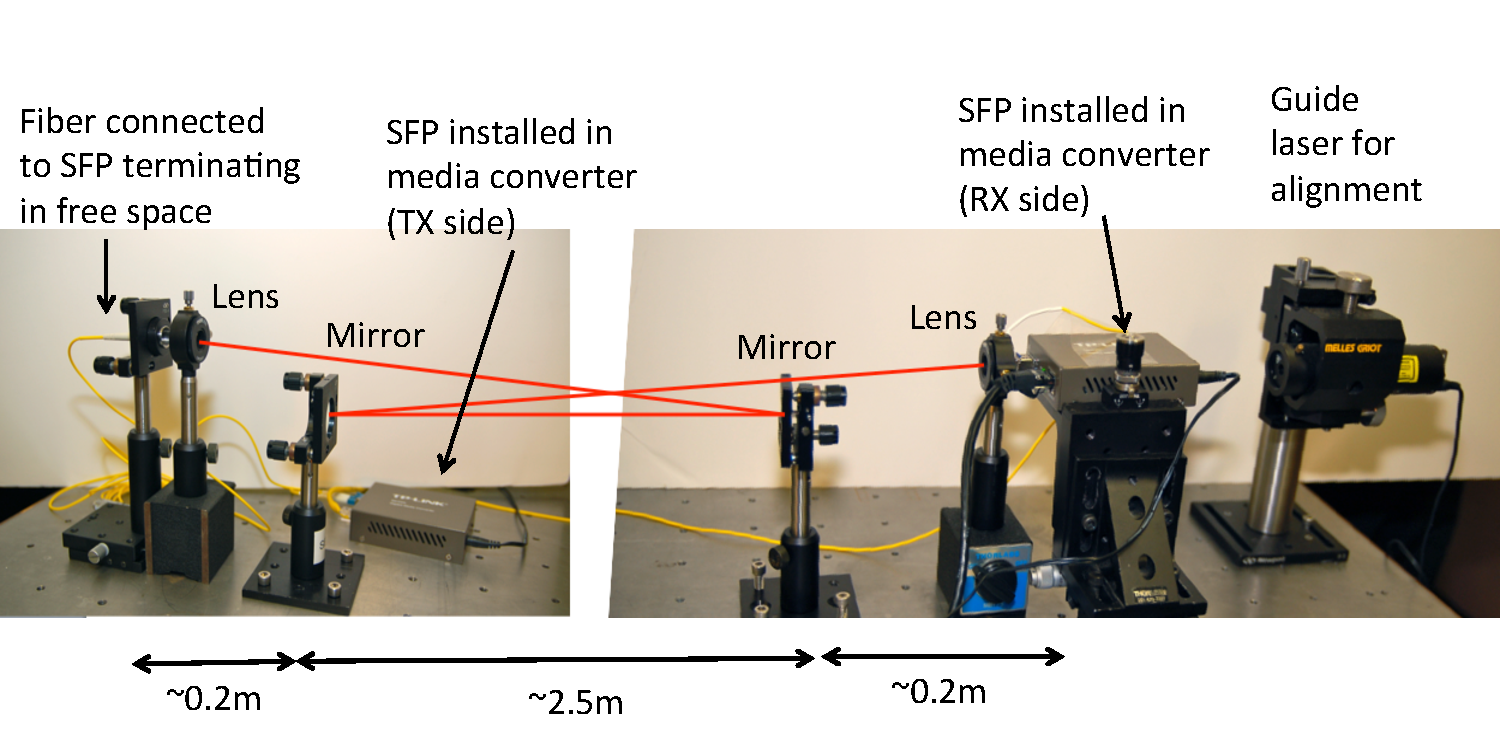
\includegraphics[width=250pt]{PPTFigs/complete-optical-setup-fig.pdf} 
%\vspace{-0.8in}
} 
\hspace*{0.3in}
\subfloat[Throughput stability]
{
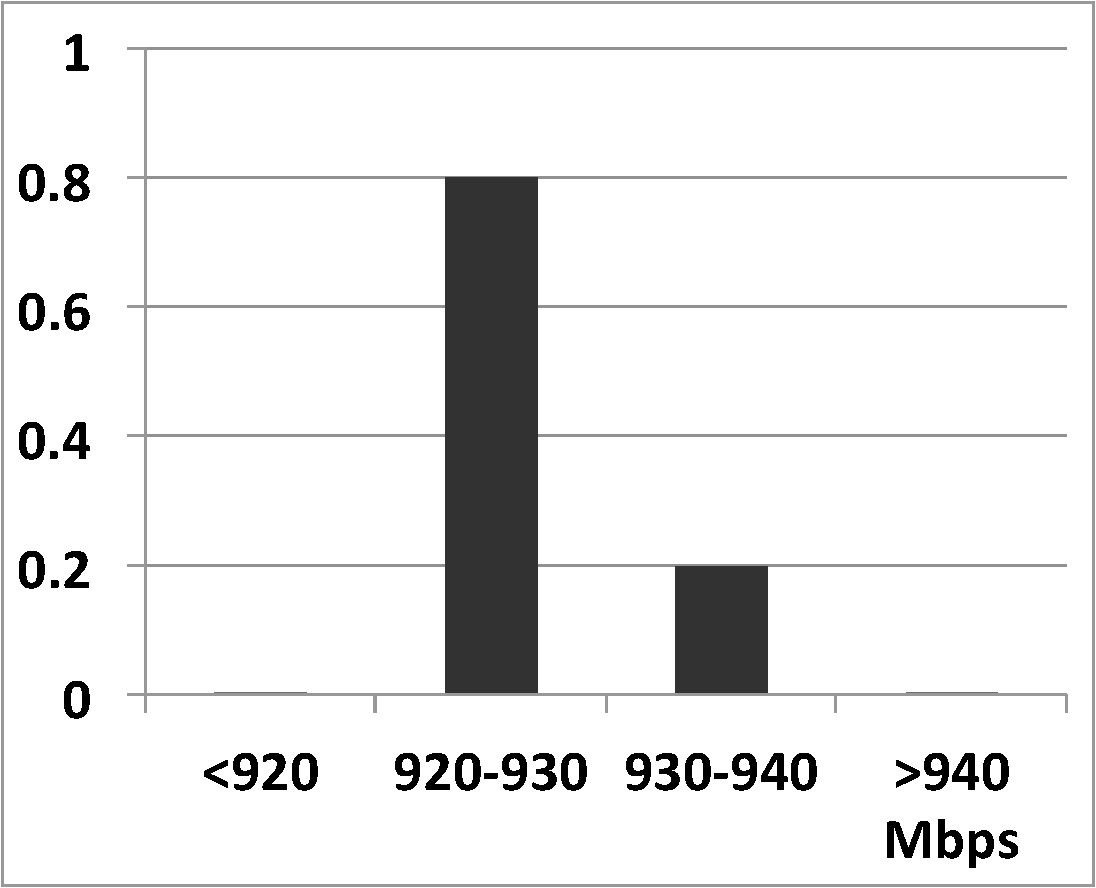
\includegraphics[width=100pt]{Figures/link-thrpt.pdf} 
}
\caption{(a) Experimental prototype showing FSO communication using SFP over ~7.5m.
Note use of mirrors to achieve a long beam path on a standard size optical bench. (The beam is hand drawn.) 
(b) Distribution
of per-second TCP throughputs (in Mbps) over a continuous 30 hour period over ~7.5m.}
\label{fig:optics-layout}
%\end{wrapfigure}
\end{figure}

\para{Preliminary Prototype of FSO Links (1Gpbs over 7.5m, with a
 misalignment-tolerance of 0.7mm).}  We have developed a
proof-of-concept prototype to demonstrate feasibility of designing
FSOs from optical SFPs. See Figure~\ref{fig:optics-layout}.  The
prototype uses a pair of 1Gbps SFPs using 1310nm lasers.  We launch
the beam from a single-mode optical fiber connected to the TX SFP on
one end \blue{with the other end terminating in free space.}  Due to
the narrow fiber diameter ($8-10 \mu\mbox{m}$), the initial beam
divergence is very large. We collimate the beam to a roughly 4mm
diameter \blue{cylinder} using an achromatic doublet lens, with the
fiber tip positioned precisely (using optical bench and translating
mounts) at the focal point of the lens. The collimated beam propagates
to a distance of 7.5m (after reflection through multiple mirrors) and
is refocussed using an identical lens on the RX
detector.\footnote{Since the SFP used here uses two separate optical
  paths (for duplex operation), the return link is closed using a
  regular fiber.} We connect the SFPs to laptops via standard media
converters~\cite{} and run TCP throughput experiments for 30 hours to
test link stability.  Figure~\ref{fig:optics-layout} demonstrates very
stable link performance comparable to the wired case. We also analyzed
the tolerance of our prototype to misalignment between the TX-RX, and
observed that the throughput is stable up to a transverse shift of
$\pm0.7 mm$.

\subsection{Fast and Precise Steering Mechanisms}

\begin{task}
\blue{Develop fast, precise, and cost-effective steering techniques to
  achieve reconfiguration in the inter-rack network.}
\end{task}

\smallskip

% DD, Survey
A wide spectrum of candidate solutions exist for laser beam steering
including phased array techniques~\cite{}. But most of these are not
commodity and some are subjects of active research. Feasibility and
cost-effectiveness for adapting these solutions for DCs are
unknown. For feasibility reasons, we will investigate the following
two promising candidate technologies.


\para{Switchable Mirrors.} Switchable mirrors (SMs) are made from a
special liquid crystal material which can be electrically controlled
to rapidly switch between reflection (mirror) and transparent (glass)
states at millisecond timescales~\cite{sm}. These are used in various
forms of visual aids in niche markets e.g., rear-view video mirrors.
%
Figure~\ref{fig:beam-redirect}(a) shows how we can use SMs for
steering beams. Each FSO device will be equipped with multiple SMs,
with each SM pre-aligned (part of offline pre-configuration) to target
a point on the ceiling mirror and thus, a receiving FSO. The desired
link is established by switching one of the SMs in the mirror state
and the other SMs in the transparent state. This is done at the TX as
well as the RX, but only shown at TX in the figure for clarity.  
A small-size SM is expected to have minimal cost ($<$
\$5~\cite{sm-personal}), when manufactured at scale. 

\begin{wrapfigure}{r}{0.4\textwidth}
\centering
{
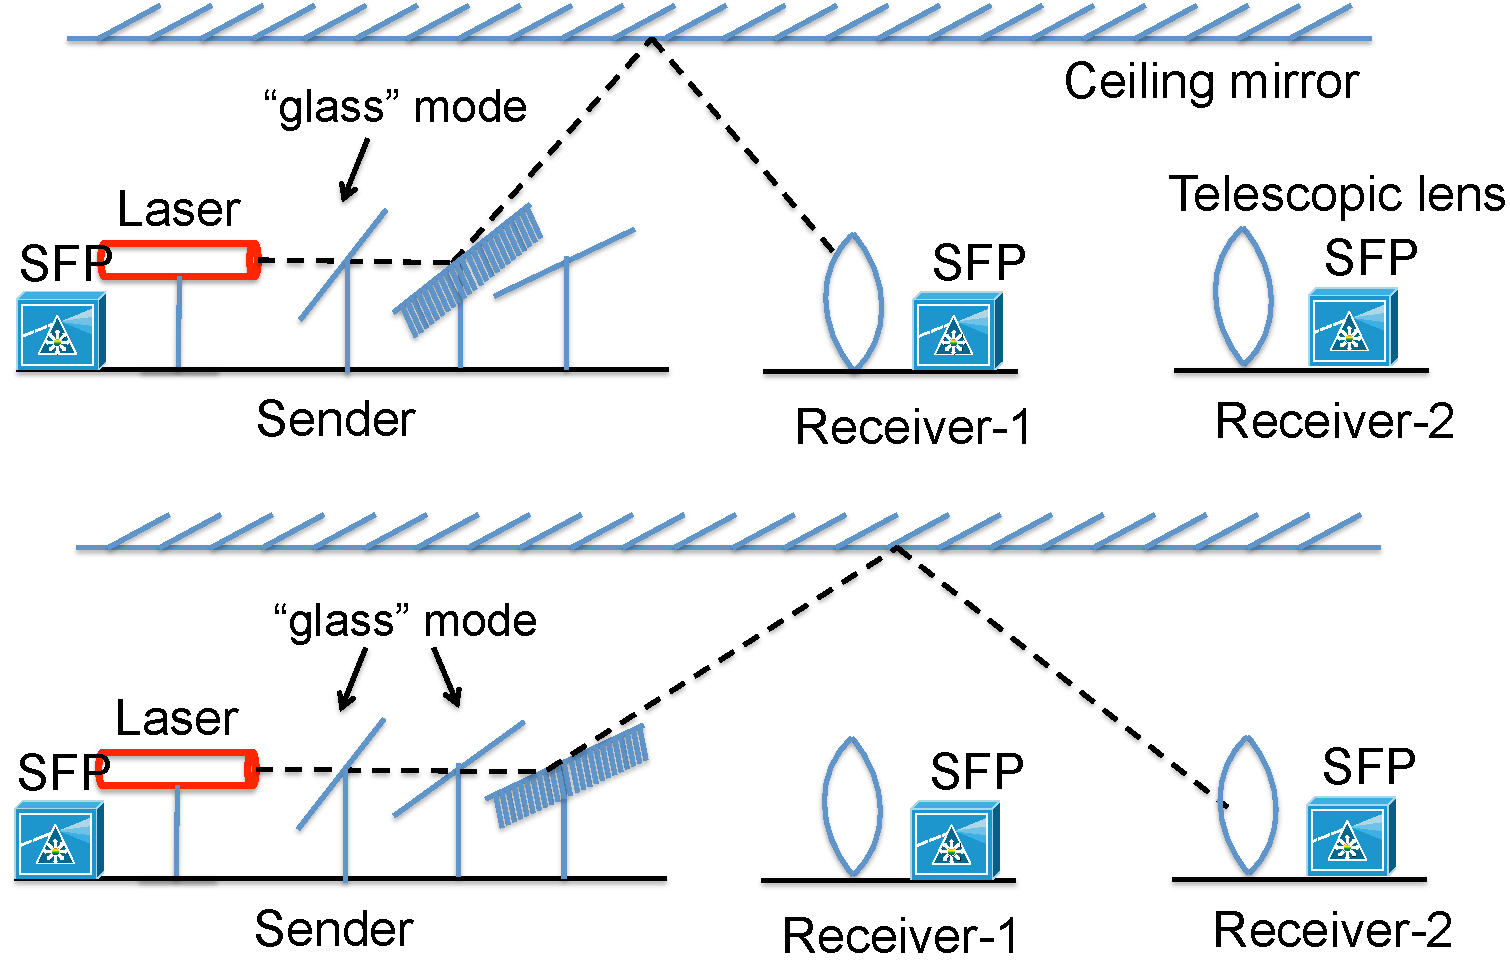
\includegraphics[width=150pt]{Figures/SM-fig.pdf} 
}
\caption{Using Switchable Mirrors with FSOs. In the top-half the
  second SM is in mirror mode, redirecting the beam to Receiver 1,
  while the bottom half has SM3 in mirror mode and thus redirecting to
  Receiver 2.}
\label{fig:beam-redirect}
\end{wrapfigure}

\softpara{Managing Minor Misalignments.} SMs are likely to require
additional mechanism to tolerate/correct minor misalignments due to
vibrations and other factors. Minimal misalignments can be tolerated
by using inexpensive vibration isolation, such as rubberized mounts
and vibration-absorption construction materials. 
%
In addition, we can use micro-positioning systems to manage minor
misalignments. Widely available piezoelectric positioning systems
would be adequate for our purposes, but they are expensive. Hence, we
would design low-cost micro-positioning mechanisms based on bimetallic
strip or other material with a high thermal expansion coefficient. By
changing the temperature of the material slightly and precisely (e.g.,
by using an electrical resistor with a varying current), we can
micro-adjust the position of the associated device. We will also
optimize the mechanical linkage and interface to maximize the range of
movement. Feedback needed for the above misalignment correction can be
obtained from the available DOM (digital opitcal monitoring) support
on optical SFPs. 

\softpara{Preliminary Study.} We evaluated the viability of switchable
mirrors using a 12" x 15" switchable mirror (SM) from Kentoptronics.
The switching latency of the SM was found to be around 250 msec.
Since the switching latency is proportional to the SM’s surface
area~\cite{sm-size}, we estimate a $<5$ msec latency for a small (1" x
1") SM we propose to use.

\para{Galvo Mirrors.} Galvo mirrors (GMs)~\cite{} are used in various
laser scanning applications. GM essentially is capable of steering a
(fixed) incident beam into a desired rectangular cone, under computer
control; this is achieved using two mirrors mounted at right
angles. See Figure~\ref{fig:beam-redirect}(b). In our context,
equipping an FSO device with a single GM enables us to target any
receiver within the \blue{pre-configured} rectangular cone (chosen
offline).

Commercially available GMs~\cite{} can provide a total rectangular
cone angle of $40^\circ$, with steering latencies of around 100
$\mu$secs. They have a pointing \blue{accuracy/precision} of within 15
$\mu$rad~\cite{} which yields a positioning error of \blue{up to 1.5mm
  for up to 100m links;} \green{this may be acceptable in our context,
  since we plan to design links with a misalignment-tolerance of up to
  4mm.}  Commodity GMs are quite large due to the associated
machinary. However, only the optical components need to remain on the
rack, while the motor and associated electronics can be hidden
underneath the rack (using custom-designed extension arms to hold the
mirrors; however, additional stability and precision issues must be
addressed). We note that emerging MEMS-based galvos~\cite{} are also
\blue{extremely} promising for the proposed concepts, and would be explored
in our research.

\softpara{Custom Building a Cost-Effective GM.}  Commodity GMs used
for laser-scanning applications are expensive (\$2000~\cite{}).
%
However, we see no reasons why the cost cannot be reduced dramatically
for our specific context. The core components of a GM include only
motor assemblies, mirrors, and some basic positioning control
capability. By using commodity hardware such as DC servo motors used
in hobby remote control aircraft and low-cost microcontrollers such as
the Arduino, we expect that \blue{extremely} high-precision control can be
obtained easily. Based on the above, we will design and build low-cost
GM prototypes for our purpose. We have a target price point of
\$30-50, when fabricated in quantity.
%
Note that the success of our research project would provide
significant motivation for additional engineering, cost-reduction, and
commoditization of GM hardware which will bring the cost
\blue{dramatically} lower.

\para{SMs vs.\ GMs.} From a \blue{mechanical perspective}, note that
SMs are physically mostly-static (after being pre-aligned), while GMs
have mirrors moving in real-time. From a topology design perspective:
a GM can reach {\em any} receiver within the \blue{prescribed} cone
(of limited angle), while use of $\NumSMsPerFSO$ SMs with an FSO
provides $\NumSMsPerFSO$ {\em arbitrary} (but fixed) target receivers.
In our research, we will systematically investigate the impact of the
above tradeoffs, and use a hybrid architecture consisting of both
steering mechanisms.  \cb

\para{Pre-Configuration.} As mentioned above, each SM needs to be {\em
  pre-aligned} to a specific receiver, and each GM needs to be {\em
  pre-oriented} to a desired rectangular cone. This is done during the
     {\em pre-configuration} phase of \ArchName; it is done offline
     (and very infrequently, e.g., monthly) using an external
     machinery, so speed and cost is not of the essence. \blue{We skip
       discussion of the required machinery and mechanisms, since it
       falls outside the scope of our project.}  However, we do
     discuss design of pre-configured topology in the following
     section.
